% ============================================================================
% !Document: IM01 [zxweather Installation Reference]
% ----------------------------------------------------------------------------
% !Revision: 001
% !IssueDate: July 2012
% !Status: Unreleased
%
% !-Classification
% !ProjectCode: DAZW [Database Applications, zxweather]
% !Type: IG [Installation Guide]
%
% !Copyright: (C) David Goodwin, 2012
% !License: FDL [GNU Free Documentation License]
% !Auhtor: David Goodwin
% ============================================================================

% Document information. This should match the above
\newcommand{\doctitle}{zxweather}
\newcommand{\docsubtitle}{Installation Reference}
%\newcommand{\projectnum}{DAZW}
\newcommand{\docnum}{IG01}
\newcommand{\docrev}{001}
\newcommand{\docdate}{July 2012}
\newcommand{\docauthor}{David Goodwin}
\newcommand{\docabstract}{This document provides installation and configuration guidelines for zxweather.}
\newcommand{\docupdateinfo}{This is a DRAFT DOCUMENT.}
\newcommand{\docosver}{Microsoft Windows NT 5.0+; Linux.}
\newcommand{\docswver}{zxweather 1.0}
\newcommand{\doccopyright}{\textcircled{c} Copyright David Goodwin, 2012.}
\newcommand{\doclicense}{Use, reproduction and modification of this document is permitted subject to the terms of the GNU Free Documentation License, Version 1.3 or any later vesion published by the Free Software Foundation. See \url{http://www.gnu.org/copyleft/fdl.html} for full license text.}

%%%%%%%%%%%%%%%%%%%%%%%%%%%%%%%%%%%%%%%%%%%%%%%%%%%%%%%%%%%%%%%%%%%%%%%%%%%%%
%                                 CONFIGURATION                             %
%%%%%%%%%%%%%%%%%%%%%%%%%%%%%%%%%%%%%%%%%%%%%%%%%%%%%%%%%%%%%%%%%%%%%%%%%%%%%

% Book type document, A4 paper, 10pt std font size:
\documentclass[a4paper,10pt,draft]{book} 

\usepackage[scaled=0.90]{helvet} % Use helvetica as the standard font
\usepackage{courier}			 % Use courier as the fixed-width font
\usepackage{hyperref}			 % Links in PDF output
\usepackage{a4wide}				 % Narrower margins for A4 documents
\usepackage{ifthen}				 % A few if statements
\usepackage{multirow}			 % Column spanning in tables
\usepackage{graphicx}			 % For pictures


% use zxtechdoc styles if they're there
\IfFileExists{zxtitle.sty}{\usepackage{zxtitle}}{}
\IfFileExists{zxtechdoc.sty}{\usepackage{zxtechdoc}}{}

\hypersetup{
    unicode=false,          % non-Latin characters in Acrobat’s bookmarks
    pdftoolbar=true,        % show Acrobat’s toolbar?
    pdfmenubar=true,        % show Acrobat’s menu?
    pdffitwindow=false,     % window fit to page when opened
    pdfstartview={FitH},    % fits the width of the page to the window
    pdftitle={\doctitle{} - \docsubtitle},    % title
    pdfauthor={\docauthor},     % author
    pdfsubject={\doctitle},   % subject of the document
    pdfkeywords={\doctitle} {\docsubtitle} {key3}, % list of keywords
    pdfnewwindow=true,      % links in new window
    colorlinks=true,       % false: boxed links; true: colored links
    linkcolor=black,          % color of internal links
    citecolor=green,        % color of links to bibliography
    filecolor=magenta,      % color of file links
    urlcolor=cyan           % color of external links
}

% Build the partnumber. Format is PROJ-DOCU.REV. If revision is 001 then it 
% is not displayed. If project is undefined it is not displayed.
\newcommand{\partnumber}{\ifthenelse{\isundefined{\projectnum}}{}{\projectnum-\docnum	\ifthenelse{\equal{\docrev}{001}}{}{.\docrev}}}

\begin{document}

% Roman Numerals for the front matter
\pagenumbering{roman}

% Setup the titlepage. We will use the zxtitle format if its there,
% otherwise the much simpler standard LaTeX one.
\ifthenelse{\isundefined{\ordernumber}}{

% Standard LaTeX titlepage
\title{\doctitle{} - \docsubtitle}
\author{\docauthor}
}{

% zxtitle titlepage
\title{\doctitle}
\subtitle{\docsubtitle}
\titleabstract{\docabstract}
\ordernumber{\partnumber}
\updateinfo{\docupdateinfo}
\osinfo{\docosver}
\swversion{\docswver}
\titlecopyright{\doccopyright}
\licensestatement{\doclicense}
}
\date{\docdate}

\maketitle

\clearpage

\tableofcontents
\clearpage

%%%%%%%%%%%%%%%%%%%%%%%%%%%%%%%%%%%%%%%%%%%%%%%%%%%%%%%%%%%%%%%%%%%%%%%%%%%%%
%                                 DOCUMENT                                  %
%%%%%%%%%%%%%%%%%%%%%%%%%%%%%%%%%%%%%%%%%%%%%%%%%%%%%%%%%%%%%%%%%%%%%%%%%%%%%

%TODO : Normalise terminology across documents (use either 'sample' or 'history record').

\chapter{Introduction}
% Back to arabac numerals for the proper content
\pagenumbering{arabic}
\setcounter{page}{1}

zxweather a collection of tools to log and display data collected from automatic weather stations compatible with the Fine Offset WH1080. It is licensed under the GNU GPL making it free software.

Its main features are:
\begin{itemize}
\item A modern HTML5 web interface
\item Basic HTML fallback for older browsers.
\item Full weather history
\end{itemize}

This manual provides installation and maintenance instructions for the entire core system. You should read this manual in its entirety to avoid problems.

\begin {figure}[!ht]
 \centering
 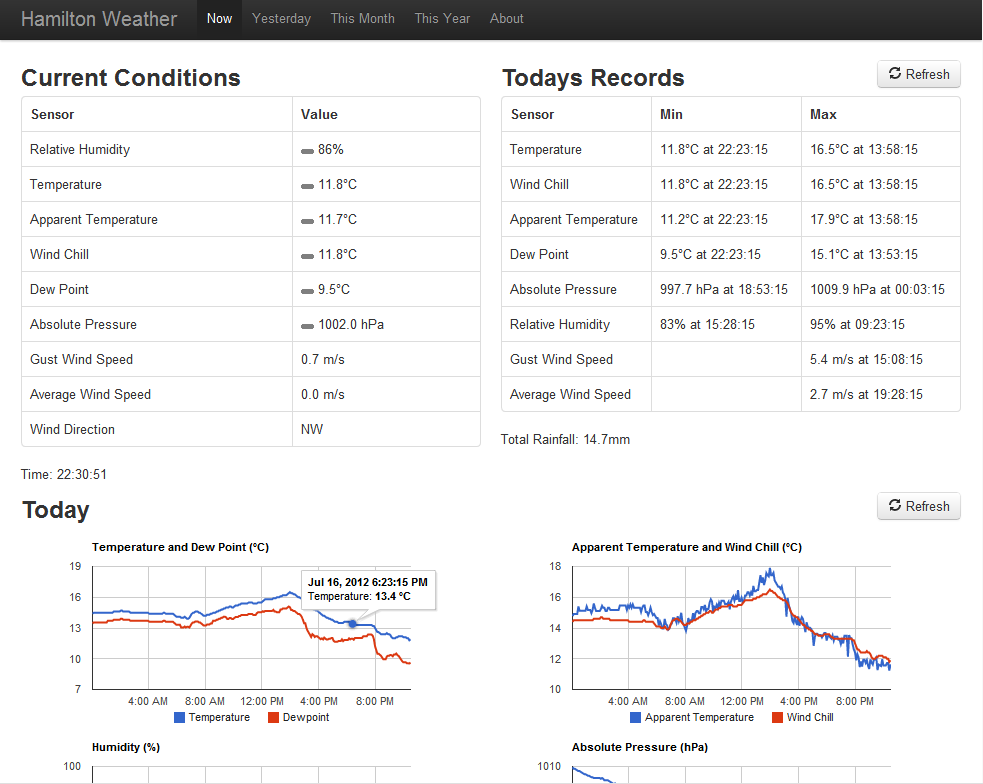
\includegraphics[scale=0.574]{images/stat_overview}
 \caption{Station Overview Page}
 \label{img_station_overview}
\end {figure}

\section{Related Documentation}
Other available documentation for the zxweather system includes:

\begin{tabular}{l l}
\verb|DAZW-WG01| & WH1080 Utilities Users Guide, version 1.0 \\
\verb|DAZW-DB01| & zxweather Database Structure, version 1.0 \\
\end{tabular}

\section{Supported Hardware}
This version of zxweather only supports weather stations 100\% compatible with the FineOffset WH1080. These weather stations are resold by many companies under various names.

The weather stations sample interval should be set to five minutes. If you have previously used software such as wview you may find your stations sample interval is set to one minute - this is not supported and will not work.

Intervals larger than five minutes should work but there may be minor issues in the web interface.

\section{System Requirements}
Linux is the recommended operating system for running the core components of zxweather. Where this is not practical it is possible to run under Microsoft Windows.

The only supported database engine is PostgreSQL. Any version from 9.0 and up should be suitable. Older versions may work but this is not tested. Other RDBMS (such as MySQL) are not supported in any way.

The WH1080 tools are only supported on little-endian CPU architectures at this time. This includes Intel IA32 (x86) and most ARM processors. Bad things will happen if your processor is big-endian.

\subsection{Software Environment}
This section covers the software environment required to run two of the core parts of the zxweather system. For PostgreSQL system requirements consult its documentation.

\subsubsection{WH1080 Utilities}
The WH1080 Utilities require the following libraries to be installed on your system:
\begin{itemize}
\item libusb-1.0 (on linux only)
\item libecpg (A part of ECPG)
\item libpq (PostgreSQL client library)
\end{itemize}

Additionally, to compile these you will need:
\begin{itemize}
\item GNU C Compiler and GNU Make
\item ECPG tool (a part of PostgreSQL)
\item Development packages for libusb-1.0 and libecpg
\end{itemize}

This software and libraries should be available from your operating systems package manager. On Debian 6.0 the packages would be \verb|build-essential| \verb|libusb-1.0-0-dev| \verb|libecpg-dev|.

\subsubsection{Web Interface}
The web interface requires the following to be installed on your system:
\begin{itemize}
\item Python 2.6 or 2.7
\item The following python libraries: 
\begin{itemize}
\item Psycopg2
\item web.py
\item python-gnupg
\item requests (if database replication is used)
\end{itemize}
\item Gnuplot
\item GnuPG (if database replication is used)
\item Apache2 with mod\_wsgi (or another web server with WSGI support)
\end{itemize}

\subsection{System Structure}
zxweather consists of three major components:
\begin{itemize}
\item Database (run on PostgreSQL)
\item Data Logger (wh1080d) and other WH1080 utilities
\item Web Interface
\end{itemize}

The database sits at the center of the zxweather system. The Data Logger feeds data into the database where the web interface and other clients can access it.

Because of this architecture all systems must be on the same network as the database server (using either SSH tunnels or VPNs). This can make running the Web Interface on a remote system (such as a VPS) difficult.

To support this sort of configuration the Web Interface as a very basic database replication facility built into it. This allows it to have its own database with weather data being pushed out to it at regular intervals.

This sort of configuration is described in more detail in Chapter \ref{cha_db_replication}.

\subsection{Data logger}
The data collection tools are written in the C language and are portable to both Linux and Windows.

ECPG (a PostgreSQL utility), GCC and GNU Make are required to compile the software. To run it, libecpg and (on linux) libusb-1.0 are required.

\subsection{Web interface}
The web interface requires Python version 2.6 or 2.7 with the following packages:
\begin{itemize}
\item Jinja2
\item web.py
\item psycopg2
\item python-gnupg
\end{itemize}

Additionally, gnuplot must be available on the system running the weatherplot program. If database replication is being used (chapter \ref{cha_db_replication}) then GnuPG must also be available.

\chapter{Database}
\label{cha_database}
% Instructions for how to setup the database. This includes permissions
% required, etc.

This chapter describes the database setup required by zxweather. The database is required by the core system and is not optional. It must be setup on a system that all other components have network access to.

Alternatively, if it is impractical for all systems to have direct access to the database it is possible to setup a second replica database on the system running the Web Interface. Chapter \ref{cha_db_replication} covers this setup in more detail.

\section{Installation}

%TODO Come up with a better database setup system. Write a python program or something. Should be able to handle database upgrades and (when the feature is added) setting up the weather station in the database.

The zxweather database has only been tested with PostgreSQL version 9.0 and above. This documentation assumes you already have a suitable version of the server and client tools installed on your system.

This section documents creating the zxweather using the command-line PostgreSQL tools. If you are more comfortable with the pgAdmin III GUI tool you may use that instead.

\subsection{Create Database}
To create the weather database, execute a command such as the following:

\begin{verbatim}
$ createdb -h dbserver -U username weather "Weather database"
\end{verbatim}

Where:
\begin{itemize}
\item \emph{dbserver} is the hostname (or IP Address) of the machine running PostgreSQL.
\item \emph{username} is the username to login to the server with. This will often be something like "postgres". The account being used must have the \emph{CREATEDB} permission.
\item \emph{weather} is the name of the new database.
\item \emph{"Weather Database"} is a description of the database. This is optional.
\end{itemize}

More information on the createdb program can be found at \url{http://www.postgresql.org/docs/9.1/static/app-createdb.html}.

\subsection{Create Database Structure}
The database structure needed by zxweather to store data is created using the \verb|database.sql| located in the \emph{database} directory of the zxweather distribution. Running this SQL script will create the full database structure in one step.

You can run this script with a command such as the following inside the zxweather distribution directory:
\begin{verbatim}
$ psql -h dbserver -U username -d weather -f database/database.sql 
\end{verbatim}
The supplied parameters are:
\begin{itemize}
\item \emph{dbserver} - The hostname (or IP Address) of the machine running PostgreSQL
\item \emph{username} - The user account to login to the server with. Using a superuser account (often called "postgres") will be easiest.
\item \emph{weather} - The name of the database you created in the previous section.
\end{itemize}

\section{Permissions}
Four programs will be accessing the database. They require user accounts with the following permissions on the weather database:

\begin{tabular}{l l}
\hline
\textbf{Program} & \textbf{Permissions} \\
\hline
wh1080d & CONNECT, SELECT, INSERT, UPDATE \\
wh1080 & CONNECT, SELECT, INSERT \\
weatherplot & CONNECT, SELECT \\
web interface & CONNECT, SELECT \\
\hline
\end{tabular}

You can create individual accounts for each program or have them all sharing the same account.

If the database replication feature in the Web Interface is being used then its user account will need the INSERT and UPDATE permissions in addition to those described in the table above.

\subsection{Creating Accounts}
%TODO Instructions for creating the accounts

\chapter{Data Logger}
% Compiling and installing wh1080d or the other program

The Data Logger is a daemon which continuously downloads weather data (both live and historical samples) from the weather station and loads it into the database. It is called wh1080d and is one of the WH1080 Utilities. Its full documentation is contained in the \emph{WH1080 Utilities Users Guide, version 1.0} (\verb|DAZW-WG01|).

This chapter covers how to compile and install this tool. Additionally, section \ref{sec_loading_data} includes some important maintenance information that must always be taken into consideration before you start wh1080d.

\section{Compiling}
This section only covers compiling the tools under Linux. If you are using Microsoft Windows it is recommended that you use the pre-compiled executables and skip to the next section.

\subsection{Requirements}
To compile the tools under Linux the following software must be installed:
\begin{itemize}
\item GNU Make
\item GNU C Compiler
\item ECPG (a PostgreSQL utility)
\end{itemize}

The following libraries are also required:
\begin{itemize}
\item libpq (PostgreSQL client library)
\item libecpg (library for ECPG)
\item libusb-1.0
\end{itemize}

These libraries and software packages should be available from your operating systems package manager. On Debian 6.0 the packages would be \verb|build-essential libusb-1.0-0-dev libecpg-dev|.

\subsection{Compiling the WH1080 Tools}

%TODO Switch to the GNU Build System and rewrite this.

To compile the WH1080 tools, cd into the wh1080 subdirectory of the zxweather distribution and run \verb|make|. This should kick off the build process and leave you with a handful of programs.

\section{Loading Data}
\label{sec_loading_data}

Before you can start the wh1080d it is important to note that you may have to run a \emph{Full Update} first. Doing this prevents issues such as:
\begin{itemize}
\item Corrupt data being inserted into the database
\item New data on the weather station from being lost
\end{itemize}

However, if the a Full Update is performed when it is \emph{not} necessary it will result in duplicate samples being inserted into your database.

\subsection{When to perform a Full Update}
There are only three occasions when it is acceptable (and necessary) to perform a full update:
\begin{itemize}
\item You have just erased the weather stations memory
\item You have reset the weather station
\item The database is more than 4080 samples out of date
\end{itemize}

The first two deal with the case where the sample the database says needs to be downloaded next no longer exists on the weather station. This prevents invalid data from being inserted into the database.

The third deals with the case where sample the database says needs to be downloaded next is not correct because \emph{all} samples needed to be downloaded. Failing to perform a full update in this case will likely result in some of the samples on your weather station being missed.

As an example, if your weather station is set to take one sample every five minutes then the database must be more than 340 hours out of date (that is a little over 14 days).

If in any doubt perform a full update on a test database and compare what it download with what is already in your weather database to see if there is any overlap at all.

\subsection{Performing a Full Update}
To perform a full update you must use the the wh1080 as wh1080\textbf{d} can not perform this operation. wh1080 is one of the WH1080 Utilities and is a basic tool for inspecting the contents of the weather station and downloading samples into a database.

The \verb|-l| command-line option causes the Update Tool to perform a Full Update instead of a regular one:

\verb|wh1080 -l -d databasename@hostname -u username -p password|

This is covered in more detail in Section 2.2.4 of \emph{WH1080 Utilities Users Guide} (DAZW-WG01).

\section{wh1080d Configuration}
\subsection{Linux}

wh1080d takes the following arguments:

\begin{tabular}{l l p{10cm}}
\hline
\textbf{Argument} & \textbf{Parameter} & \textbf{Description} \\
\hline
-d & database & Database connection string \\
-u & username & Database username \\
-p & password & Database password \\
-f & filename & Log file to write messages to \\
\hline
\end{tabular}

Under linux the Update Service runs as a daemon. To start it just run something like the following from your system startup scripts:

\verb|wh1080d -d database -u username -p password -f logfile|

The log file is truncated when the daemon starts.

\subsection{Windows}

%TODO Add the ability to run wh1080d as a windows service and document it here.

\chapter{Web Interface}

The Web Interface is the primary way for viewing data in the zxweather database. It consists of two components - the WSGI web application and the chart plotting program.

Both components are required for correct operation. This chapter describes how to install and configure them.

% Overview of features

\section{WSGI Application}

The web interface is written as a Python WSGI application. This section only covers installing the application under Apache httpd. If you are not using Apache then consult your web servers documentation for instructions on installing wsgi applications.

\subsection{Installation}
% Where to put it
% Apache configuration

At this time zxweather cannot be run in a subdirectory - it must live in the root directory of the website. This generally means giving it its own virtual host.

The system you are installing the web interface on must have the following installed on it:
\begin{itemize}
\item Apache httpd
\item mod\_wsgi
\item Python 2.6 or 2.7 with the following packages:
\begin{itemize}
\item psycopg2
\item web.py
\item python-gnupg
\end{itemize}
\end{itemize}

Installation and configuration of these packages is outside the scope of this document. If you are setting up on a Linux system the packages are likely all available from your distributions package repositories. 

Where examples are provided in this section they are for Debian-based Linux distributions. Installation and configuration on Windows systems is similar but requires more effort.

\subsubsection{Extract Distribution}
Firstly if you haven't already done so extract the full zxweather distribution to some location on your disk. In the examples \\ /opt/zxweather is used:
\begin{verbatim}
$ pwd
/opt/zxweather
$ ls
database  doc  index.txt  plot  wh1080  zxw_web
\end{verbatim}

\subsubsection{WSGI Setup}
As the zxweather web interface is a Python WSGI application you must have the mod\_wsgi installed and enabled. On Debain-based systems the package is called \verb|libapache2-mod-wsgi| and can be enabled using the \verb|a2enmod| tool:

\begin{verbatim}
$ a2enmod wsgi
\end{verbatim}

\subsubsection{Virtual-host Configuration}

All that is required to make zxweather work from the Apache end is adding the following to your vhost configuration file:
\begin{verbatim}
WSGIScriptAlias / /opt/zxweather/zxw_web/zxweather.py
\end{verbatim}

An example virtual host configuration might look like this:

\begin{verbatim}
<VirtualHost *:80>
        ServerAdmin admin@example.com
        ServerName weather.example.com

        DocumentRoot /var/www
        ErrorLog ${APACHE_LOG_DIR}/weather-error.log
        LogLevel warn
        CustomLog ${APACHE_LOG_DIR}/weather-access.log combined

        WSGIScriptAlias / /opt/zxweather/zxw_web/zxweather.py
</VirtualHost>
\end{verbatim}

\subsection{Configuration}
% The configuration file

The Web Interface attempts to load a configuration file with one of the following names when it starts:

The Web Interface attempts to load configuration files in the following order. Only the first one it finds is loaded.
\begin{itemize}
\item \verb|config.cfg| (in the current directory)
\item \verb|zxw_web/config.cfg|
\item \verb|/etc/zxweather.cfg|
\end{itemize}

It is recommended that you install your configuration file in \verb|/etc|. To do this, copy the \\ \verb|zxweather.cfg.sample| file included in the zxweather distributions \verb|zxw_web| subdirectory:
\begin{verbatim}
$ cp /opt/zxweather/zxw_web/zxweather.cfg.sample /etc/zxweather.cfg
\end{verbatim}

This configuration files format is similar to the INI format commonly used on Microsoft Windows. The '\#' character marks a comment, group names are inside square brackets.

\subsubsection{Database}
The first group is for database configuration. It looks like the following:
\begin{verbatim}
[database]
host: localhost
port: 5432
database: weather
user: weatheruser
password: password
\end{verbatim}

Where the settings are:
\begin{itemize}
\item host - the hostname or IP address of your database server.
\item port - The port your database listens on. This is commonly 5432 for PostgreSQL.
\item database - Name of your database.
\item user - The user to login to the server as
\item password - The users password.
\end{itemize}


\subsubsection{Data}
The Data group stores details about the data available in your database:

\begin{verbatim}
[data]
live_data_available: True
sample_interval: 300
plot_interval: 1800
\end{verbatim}

The settings are:
\begin{itemize}
\item live\_data\_available - If Live Data is available from the database. If you are using wh1080d to populate your database then this should be left as \verb|True|
\item sample\_interval - How often new samples appear in the database (in seconds). Only a 5 minute sample interval is supported at the moment so this should be left as 300
\item plot\_interval - How often the weatherplot program runs (see section \ref{sec_chart_plotting}) in seconds. 
\end{itemize}

\subsubsection{Site}
The Site group stores basic web interface configuration:
\begin{verbatim}
[site]
default_ui: s
site_name: zxweather
# UNCOMMENT THESE AND SET THEM! The defaults will NOT work.
#site_root: http://weather.example.com/
#static_data_dir: /var/weather/static/
#station_name: abc
\end{verbatim}

Where the settings are:
\begin{itemize}
\item default\_ui - The default UI to use. 's' is the Standard UI, 'b' is the Basic (HTML-only) UI. Unless your only browser is from 2001 you will want to leave this on 's'.
\item site\_name - The name of your site. This appears on the left of the navigation bar and in the title of every page.
\item site\_root - The URL for the root of your website. For example, http://weather.example.com/.
\item static\_data\_dir - Where on your hard disk the static data directory is. If zxweather was extrated to \verb|/opt/zxweather| then this should be set to \verb|/opt/zxweather/zxw_web/static/|.
\end{itemize}

The final setting in this group is station\_name. This is a very short (a few characters) name for your weather station. It should be kept very short as it will appear in the URL of every page in your site. For example, if you set this value to "foo" your station overview page will be \verb|http://weather.example.com/s/foo/|.

The purpose of this setting is to allow multiple weather datasets to be handled by a single Web Interface instance in a future version of zxweather. Uses for this functionality may be:
\begin{itemize}
\item Multiple weather stations.
\item Separating datasets if you move the weather station to a different location.
\end{itemize}

Once you have chosen a value for this setting you should never change it as it will change every URL in your site.

\subsubsection{database\_replication}
This group configures the database replication feature. If you do not plan on using this feature then the default values (which turn the feature off) are acceptable.

If you are going to use this feature then these settings are described in Chapter \ref{cha_db_replication}.

\subsection{About Page}
% About page
On the navigation bar of the standard Web Interface is an "About" link which will take you to a generic about page which you will want to customise.

To do this, navigate into the \emph{static data} directory ( \verb|/zxw_web/static/|) and copy the \verb|about.html| file into your weather stations subdirectory. If, for example, your station is called "foo" and zxweather is installed in \verb|/opt/zxweather| you would copy \verb|/opt/zxweather/zxw_web/static/about.html| to \\ \verb|/opt/zxweather/zxw_web/static/foo/about.html|. You can then customise this copy of the file. You should avoid modifying the original copy as it may be overwritten without warning by future versions.

When editing your copy of \verb|about.html| you will find two comments near the bottom of the page; \\
\verb|<!-- BEGIN_USER_CONTENT -->| and \verb|<!-- END_USER_CONTENT -->|. You can put anything you want between these comments.

It is best to avoid making any changes outside of these comments as future versions may make changes to the file outside these comments as part of the upgrade process.


\section{Chart Plotting}
\label{sec_chart_plotting}
% Purpose of this program
% Command-line arguments
% How to set it up

The \verb|weatherplot| program is responsible for generating static charts primarily used by the basic HTML web interface. It must be setup as a scheduled task to be run at regular intervals.

The machine it runs on must have \emph{gnuplot} installed and must have access to the database server and directory the zxweather web interface runs from.

\subsection{Usage}

The weatherplot program is written in the Python language and lives in the \verb|plot| subdirectory of the zxweather distribution. It is executed on the command-line with python as: \\ \verb|$ python plot/weatherplot.py [arguments]|.

The charts it generates must be put in the web interfaces \emph{static data} directory in a subdirectory with the same name as your station. For example, if your station is named "foo" and the zxweather distribution was extracted to \verb|/opt/zxweather| then you would generate charts into \\ \verb|/opt/zxweather/zxw_web/static/foo/|.

By default an executable called \verb|gnuplot| is expected to be in the path which it can use to generate the charts. If your install of gnuplot is not in the path or goes by another name use the \verb|--gnuplot-binary| parameter to specify its name.

\subsubsection{Example}
This example regenerates \emph{all} charts for all data in the database. It is run from the zxweather directory.
\begin{verbatim}
$ python plot/weatherplot.py --directory zxw_web/static/foo/ \
-t weather -n localhost -u postgres -p password
\end{verbatim}

If your install of gnuplot is not in the path or is not called \verb|gnuplot| then you would supply the \\ \verb|--gnuplot-binary| argument:
\begin{verbatim}
$ python plot/weatherplot.py --directory zxw_web/static/foo/ \
-t weather -n localhost -u postgres -p password \
--gnuplot_binary /opt/gnuplot/bin/gnuplot-custom-build
\end{verbatim}

\subsubsection{Command-line Arguments}
The weatherplot program accepts the following command-line arguments:

\begin{tabular}{p{3.4cm} l p{8cm}}
\hline
\textbf{Argument} & \textbf{Parameter} & \textbf{Description} \\
\hline
\verb|-t| \par \verb|--database| & dbname & Name of the database to use. Required. \\
\verb|-n| \par \verb|--host| & hostname & Database server hostname. Required. \\
\verb|-u| \par \verb|--user| & username & Username for database server. Required. \\
\verb|-p| \par \verb|--password| & password & Password for database server. Required. \\
\verb|-d| \par \verb|--directory| & directory & Output directory. Required. \\
\verb|-a| \par \verb|--plot-new| & filename & Only plots charts for dates on or after that stored in the specified file. \\
\verb|-r| \par \verb|--replot-pause| & seconds & Number of seconds to wait before replotting.\\
\verb|-g| \par \verb|--gnuplot-binary| & filename & Name of the gnuplot executable to use.\\
\hline
\end{tabular}

The database, host, user, password and directory parameters are always required.

\subsection{Plotting All Charts}

To regenerate charts for your entire database run the weatherplot program with only the minimum command-line arguments:

\begin{verbatim}
$ python plot/weatherplot.py --database weather --host localhost \
--user postgres --password password \
--directory zxw_web/static/station_name/
\end{verbatim}

This will create charts for all days and months in your database and store them in the specified directory. Depending on the size of your database this may take some time.

Some software upgrades may require you to do this when new chart types have been added or the style of the charts has been adjusted.

\subsection{Running as a Scheduled Task}

The recommended way to setup the weatherplot program is to run it as a scheduled task from cron or the windows task scheduler. When run in this way it is important that it be set to only plot charts containing new data.

The \verb|--plot-new| command-line argument implements this. The argument takes a single parameter which is the name of a file to store the date of the last plotted day in.

Each time the weatherplot program is executed with this parameter it will replot all charts for all days and months on or after the date in that file and then update the file with todays date. That way only charts that need to be regenerated are regenerated.

\subsubsection{Example}

When run as below weatherplot will only replot charts that have changed since it was last run:
\begin{verbatim}
$ python plot/weatherplot.py --database weather --host localhost
--user postgres --password password --directory static/station_name/
--plot-new plot_status_file
\end{verbatim}

To make this run every 30 minutes you would add a line such as the following to /etc/crontab:
\begin{verbatim}
0,30 *  * * *   root    cd /var/zxweather && \
  python plot/weatherplot.py -t weather -n localhost -u postgres \
  -p password -d zxw_web/static/station_name -a plot_status_file  
\end{verbatim}

If the static charts are not important to you, you may wish to only regenerate them every few hours or once a day.

\subsection{Plotting Continuously}

The weatherplot program is capable of running interactively in continuous mode. When run like this it will automatically replot charts at a specific interval until you terminate it with Ctrl+C. This is primarily intended for testing purposes.

It can be run in this mode by supplying the \verb|--replot-pause| parameter
with a suitable interval in seconds.

\subsubsection{Example}

When run as below the behaviour is the same as setting it up to be run by cron every 30 minutes except it runs continuously attached to the terminal.

\begin{verbatim}
$ python plot/weatherplot.py --database weather --host localhost \
--user postgres --password password --directory zxw_web/static/rua \
--plot-new plot_status_file --replot-pause 1800

Weather data plotting application v1.0
        (C) Copyright David Goodwin, 2012


Connecting to database...
Server version: PostgreSQL 9.1.2, compiled by Visual C++ build 1500
Generating temperature plots in zxw_web/static/rua
Plotting from 2012-05-10
Plotting graphs for 2012...
Plotting graphs for 2012 may...
Plot zxw_web/static/rua/2012/may/temperature_tdp_large.png
Plot zxw_web/static/rua/2012/may/temperature_awc_large.png
Plot zxw_web/static/rua/2012/may/humidity_large.png
Plot zxw_web/static/rua/2012/may/indoor_humidity_large.png
Plot zxw_web/static/rua/2012/may/pressure_large.png
Plot zxw_web/static/rua/2012/may/indoor_temperature_large.png
Plot zxw_web/static/rua/2012/may/temperature_tdp.png
Plot zxw_web/static/rua/2012/may/temperature_awc.png
Plot zxw_web/static/rua/2012/may/humidity.png
Plot zxw_web/static/rua/2012/may/indoor_humidity.png
Plot zxw_web/static/rua/2012/may/pressure.png
Plot zxw_web/static/rua/2012/may/indoor_temperature.png
Plotting graphs for 2012 may 9...Skip
Plotting graphs for 2012 may 10...
Plot zxw_web/static/rua/2012/may/10/temperature_tdp_large.png
Plot zxw_web/static/rua/2012/may/10/temperature_awc_large.png
Plot zxw_web/static/rua/2012/may/10/humidity_large.png
Plot zxw_web/static/rua/2012/may/10/indoor_humidity_large.png
Plot zxw_web/static/rua/2012/may/10/pressure_large.png
Plot zxw_web/static/rua/2012/may/10/indoor_temperature_large.png
Plot zxw_web/static/rua/2012/may/10/temperature_tdp.png
Plot zxw_web/static/rua/2012/may/10/temperature_awc.png
Plot zxw_web/static/rua/2012/may/10/humidity.png
Plot zxw_web/static/rua/2012/may/10/indoor_humidity.png
Plot zxw_web/static/rua/2012/may/10/pressure.png
Plot zxw_web/static/rua/2012/may/10/indoor_temperature.png
Plot zxw_web/static/rua/2012/may/10/7-day_temperature_tdp_large.png
Plot zxw_web/static/rua/2012/may/10/7-day_temperature_awc_large.png
Plot zxw_web/static/rua/2012/may/10/7-day_humidity_large.png
Plot zxw_web/static/rua/2012/may/10/7-day_indoor_humidity_large.png
Plot zxw_web/static/rua/2012/may/10/7-day_pressure_large.png
Plot zxw_web/static/rua/2012/may/10/7-day_indoor_temperature_large.png
Plot zxw_web/static/rua/2012/may/10/7-day_temperature_tdp.png
Plot zxw_web/static/rua/2012/may/10/7-day_temperature_awc.png
Plot zxw_web/static/rua/2012/may/10/7-day_humidity.png
Plot zxw_web/static/rua/2012/may/10/7-day_indoor_humidity.png
Plot zxw_web/static/rua/2012/may/10/7-day_pressure.png
Plot zxw_web/static/rua/2012/may/10/7-day_indoor_temperature.png
Plot completed at 2012-05-10 22:31:46.953000
Waiting for 1800 seconds to plot again. Press Ctrl+C to terminate.
\end{verbatim}

\chapter{Database Replication}
\label{cha_db_replication}
% Document the db_push scripts.

\section{Security}
% Overview of signing, etc.

\section{Web Interface Configuration}

In order to use the database replication feature you must enable it in the Web Interfaces configuration file. This is done in the database\_replication group towards the end of the file:
\begin{verbatim}
[database_replication]
enable: False
#gnupg_home:
#gpg_binary:
#key_fingerprint:
\end{verbatim}

The settings here are:
\begin{itemize}
\item enable - If the feature is enabled or not. Set this to "True".
\item gnupg\_home - The location where GnuPG stores keys, etc.
\item gpg\_binary - If GnuPG is installed in an unusual location on your system, specify it here.
\item key\_fingerprint - The signing keys fingerprint. If specified then only data signed with that key will be accepted. If not specified then any data with a valid signature is accepted.
\end{itemize}

\chapter{Troubleshooting}

\section{Database Replication}
% gnupg home directory must be owned by what ever user zxw_web is running as, otherwise you get no key errors.

%%%%%%%%%%%%%%%%%%%%%%%%%%%%%%%%%%%%%%%%%%%%%%%%%%%%%%%%%%%%%%%%%%%%%%%%%%%%%
%                                END DOCUMENT                               %
%%%%%%%%%%%%%%%%%%%%%%%%%%%%%%%%%%%%%%%%%%%%%%%%%%%%%%%%%%%%%%%%%%%%%%%%%%%%%

% Back page
\newpage
\thispagestyle{empty}
\begin{flushright}
\null
\vfill
\tt \partnumber
\end{flushright}
\end{document}